\documentclass[twoside, final]{hcmut_report}

% Configuration
\upperuniname{ĐẠI HỌC QUỐC GIA THÀNH PHỐ HỒ CHÍ MINH}
\uniname{TRƯỜNG ĐẠI HỌC BÁCH KHOA}
\deptname{KHOA KHOA HỌC VÀ KỸ THUẬT MÁY TÍNH}

\coursename{Mạch điện - Điện tử}
\reporttype{Báo cáo Lab 3}
\title{Bipolar Junction Transistor}
\advisor{
    Phạm Công Thái
}
\student{
    Nguyễn Hữu Thịnh,   2313292
    Nguyễn Chí Thanh,   2313078
    Nguyễn Thái Sơn ,   2312968
}
\begin{document}
\coverpage
\pagestyle{empty}
\tableofcontents
\pagestyle{fancy}
\newpage

\section{Exercise 1}
Cho sơ đồ mạch điện sau. Tính giá trị của $v_0$ và $i$. Sau đó mô phỏng mạch để kiểm tra kết quả
\begin{figure}[!htbp]
    \centering
    \includegraphics[width=0.5\textwidth]{graphics/ex1/f1.PNG}
    \caption{}
\end{figure}

\subsection{Tính toán}

Áp dụng KVL cho loop theo chiều kim đồng hồ, ta có:
\begin{align}
    -12 + 4i +2v_0 - 4 + 6i = 0
\end{align}
Áp dụng định luật Ohm cho điện trở $6 \Omega$
\begin{align}
    v_0 = -6i
\end{align}
Từ (1.1) và (1.2), ta được:
\begin{align*}
    -16 + 10i - 12i = 0 \rightarrow i = -8 \ \text{A}
\end{align*}
và \(v_0 = 48 \ \text{V}\)

\subsection{Mô phỏng}

Kết quả mô phỏng:

\begin{figure}[!htbp]
    \centering
    \includegraphics[width=0.7\textwidth]{graphics/ex1/f2.PNG}
\end{figure}
\section{Metal Oxide Semiconductor FET}
As well as the Junction Field Effect Transistor (JFET), there is another type of Field Effect Transistor available whose Gate input is electrically insulated from the main current carrying channel and is therefore called an Insulated Gate Field Effect Transistor.

The most common type of insulated gate FET which is used in many different types of electronic circuits is called the Metal Oxide Semiconductor Field Effect Transistor or MOSFET for short.

The IGFET or MOSFET is a voltage controlled field effect transistor that differs from a JFET in that it has a “Metal Oxide” Gate electrode which is electrically insulated from the main semiconductor n-channel or p-channel by a very thin layer of insulating material usually silicon dioxide, commonly known as glass.
\subsection{Depletion-mode MOSFET}
The Depletion-mode MOSFET, which is less common than the enhancement mode types. This device is very similar to JFET, except that the maximum current saturation is obtained at VGS > 0.  The circuit used to verify IDSS and VP for DFET is presented as follows:
\begin{figure}[!htp]
    \centering
    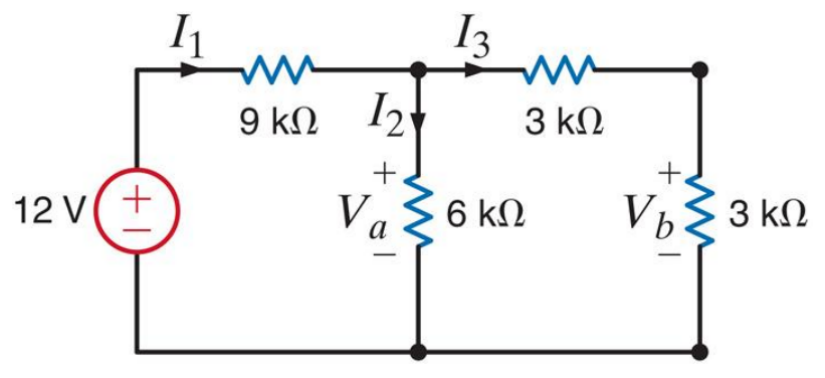
\includegraphics[width = 3in]{graphics/ex2/f1.png}
    \caption{DFET verification in PSPICE}
    \label{dfet_1}
\end{figure}
\pagebreak
The device for a common DFET is MbreakND. After a dc sweep simulation when V3 varies from -5V to 0V, the results are shown bellow:
\begin{figure}[!htp]
    \centering
    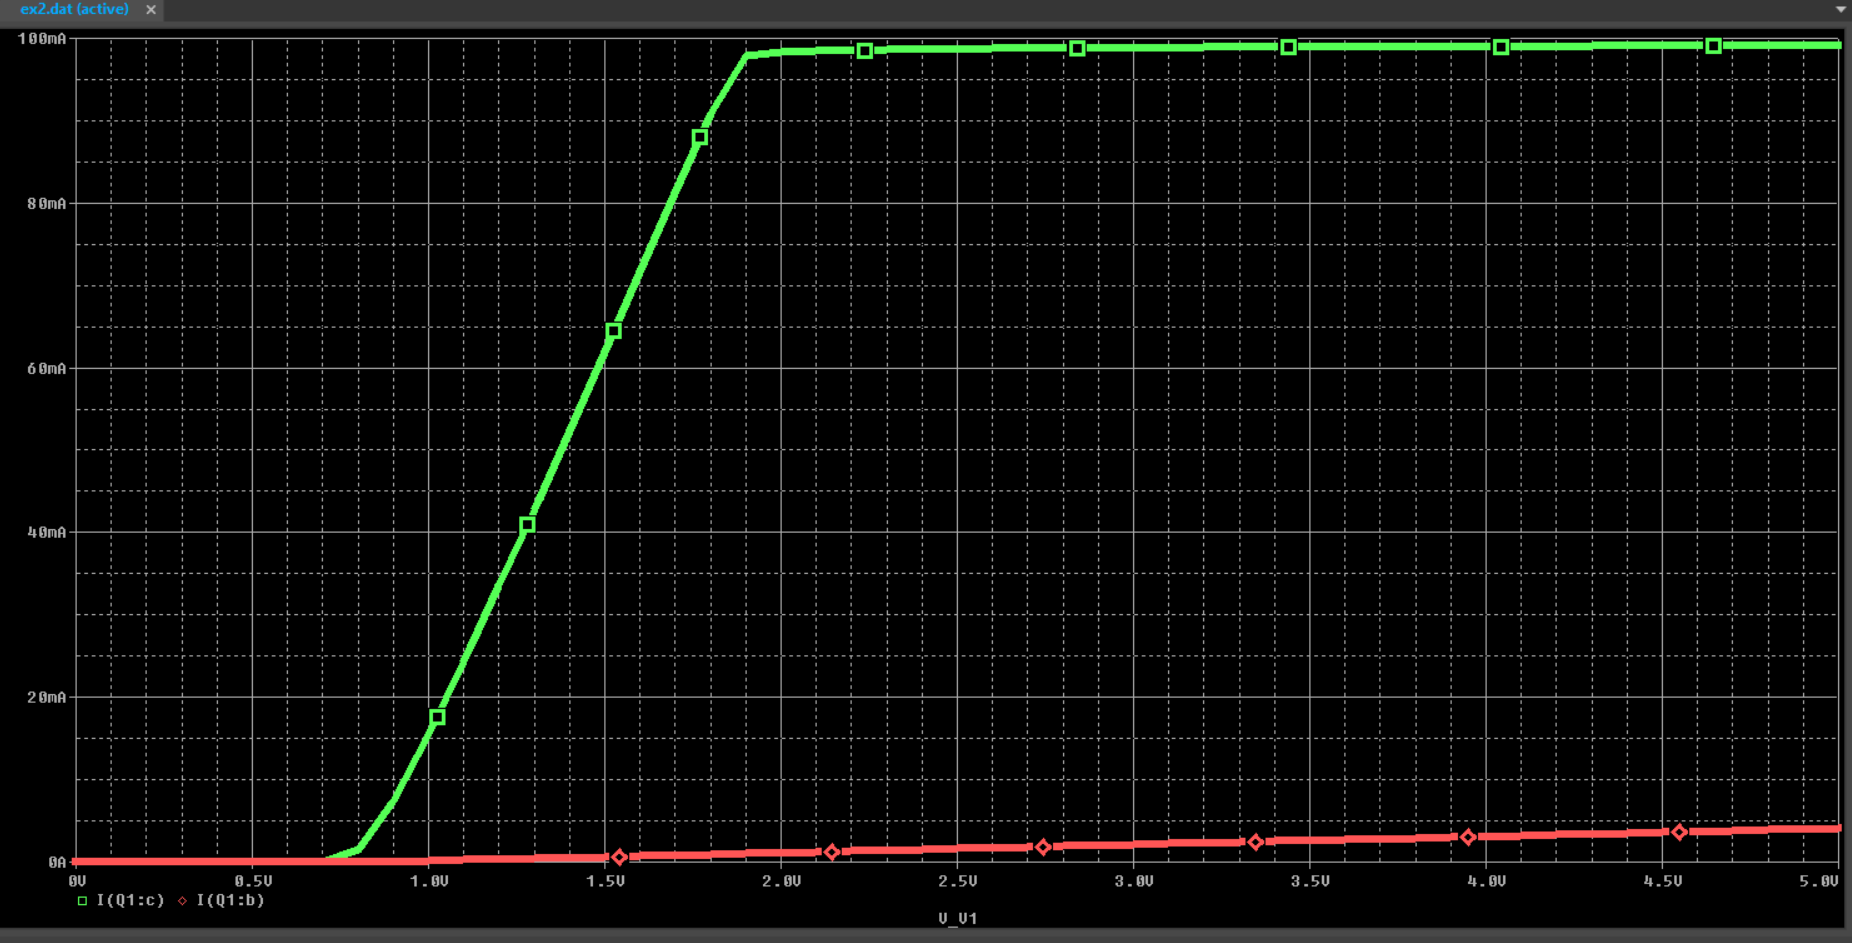
\includegraphics[width = 3in]{graphics/ex2/f2.png}
    \caption{Simulation results with DFET}
    \label{dfet_2}
\end{figure}

From this simulation results, it is confirmed that IDSS = 160mA and VP = -4V for DFET.

\textbf{Students are proposed to implement the circuit bellow:}
\begin{figure}[!htp]
    \centering
    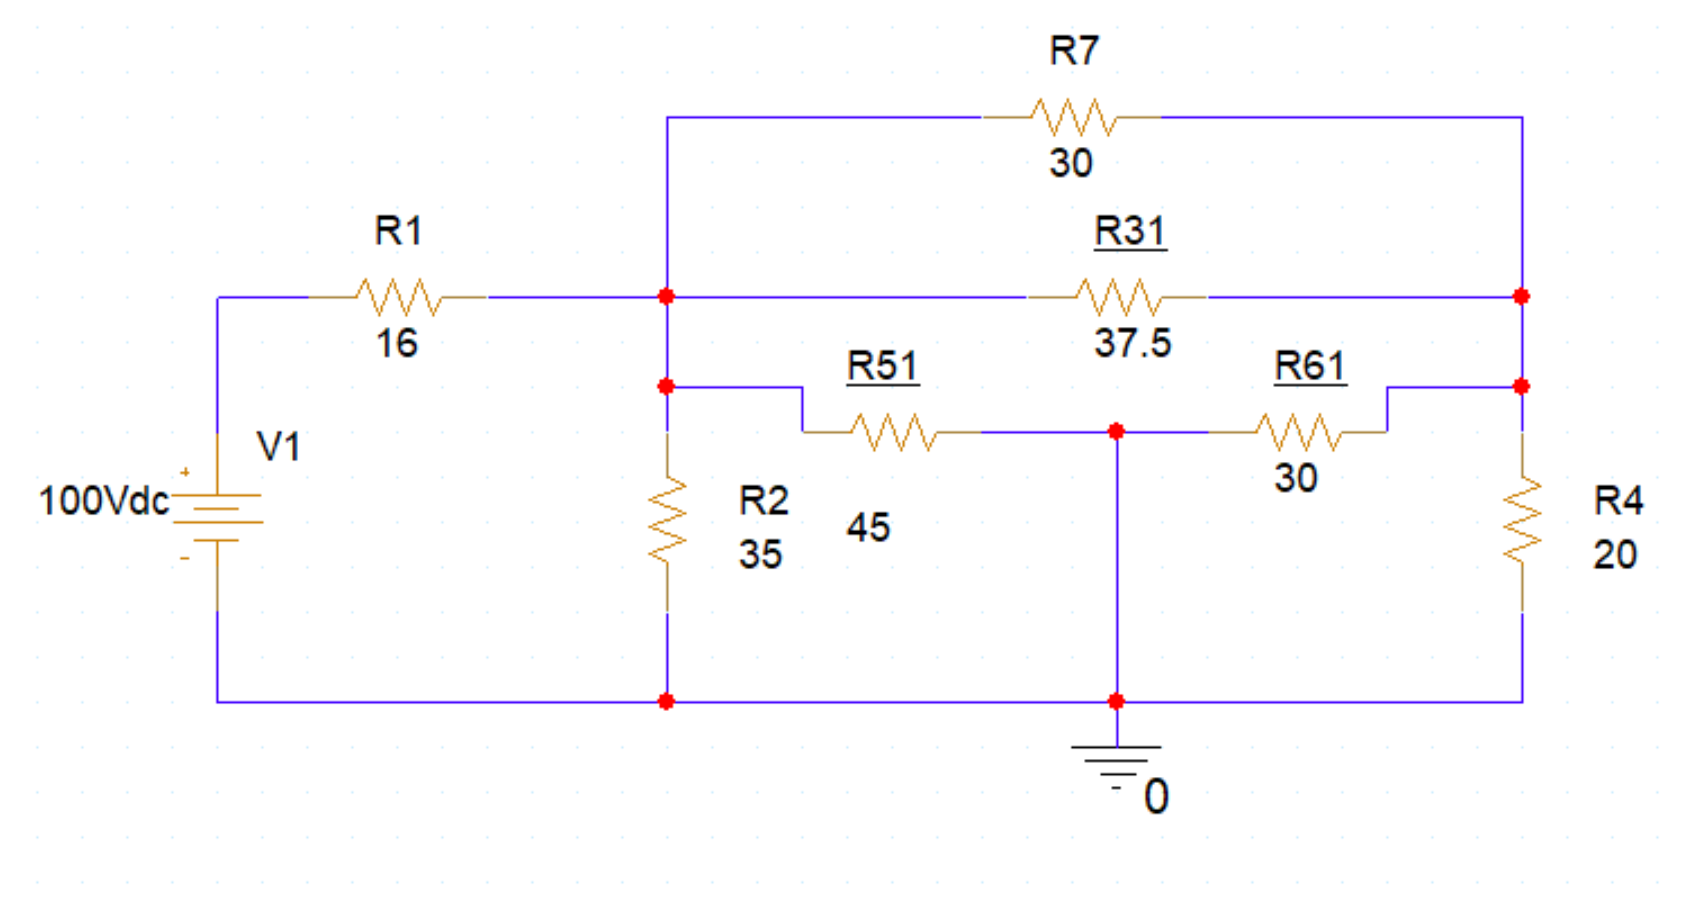
\includegraphics[width = 3in]{graphics/ex2/f3.png}
    \caption{Self bias configuration for DFET}
    \label{dfet_3}
\end{figure}



Only the bias configuration is required to executed. Please capture the simulation results with current and voltage information on the circuit. Finally, explain these values by theory cal-culations.

\textbf{a) Theory Calculation}
\begin{equation}
    I_D = I_{DSS} \left( 1 - \frac{V_{GS}}{V_P} \right)^2 \tag{1}
\end{equation}

\begin{equation}
    V_{GS} = -I_D \cdot R_S \tag{2}
\end{equation}

From equations (1) and (2), we get:
\begin{equation}
    I_D = I_{DSS} \left( 1 - \frac{-I_D \cdot R_S}{V_P} \right)^2
\end{equation}

With:
\[
    I_{DSS} = 160 \, (\mu A), \quad V_P = -4 \, (V), \quad R_S = 1 \, (k\Omega)
\]

Thus:
\[
    I_D = 107.9 \, (mA) \quad (\text{omit } I_D = 148.4 \, (\mu A) \text{due to } \, I_D > I_{DSS})
\]
\[
    V_{GS} = -148.4 \, (mV)
\]
\textbf{b) Pspice Simulation}
\begin{figure}[!htp]
    \centering
    \includegraphics[width=0.5\textwidth]{graphics/ex2/f4.PNG}
\end{figure}

\subsection{Enhancement-mode MOSFET}
The more common Enhancement-mode MOSFET or eMOSFET. The device is normally “OFF” (non-conducting) when the gate bias voltage, VGS is equal to zero. For the n-channel enhance-ment MOS transistor a drain current will only flow when a gate voltage ( VGS ) is applied to the gate terminal greater than the threshold voltage ( VTH ) level in which conductance takes place making it a transconductance device. In other words, for an n-channel enhancement mode MOSFET: +VGS turns the transistor “ON”, while a zero or -VGS turns the transistor “OFF”. Thus the enhancement-mode MOSFET is equivalent to a “normally-open” switch.

The reverse is true for the p-channel enhancement MOS transistor. When VGS = 0 the device is “OFF” and the channel is open. The application of a negative (-ve) gate voltage to the p-type eMOSFET enhances the channels conductivity turning it “ON”. Then for an p-channel enhancement mode MOSFET: +VGS turns the transistor “OFF”, while -VGS turns the transistor “ON”.

The validation of an EFET in PSPICE is presented bellow. The typical EFET in PSPICE is \textbf{MbreakN} device.
\begin{figure}[!htp]
    \centering
    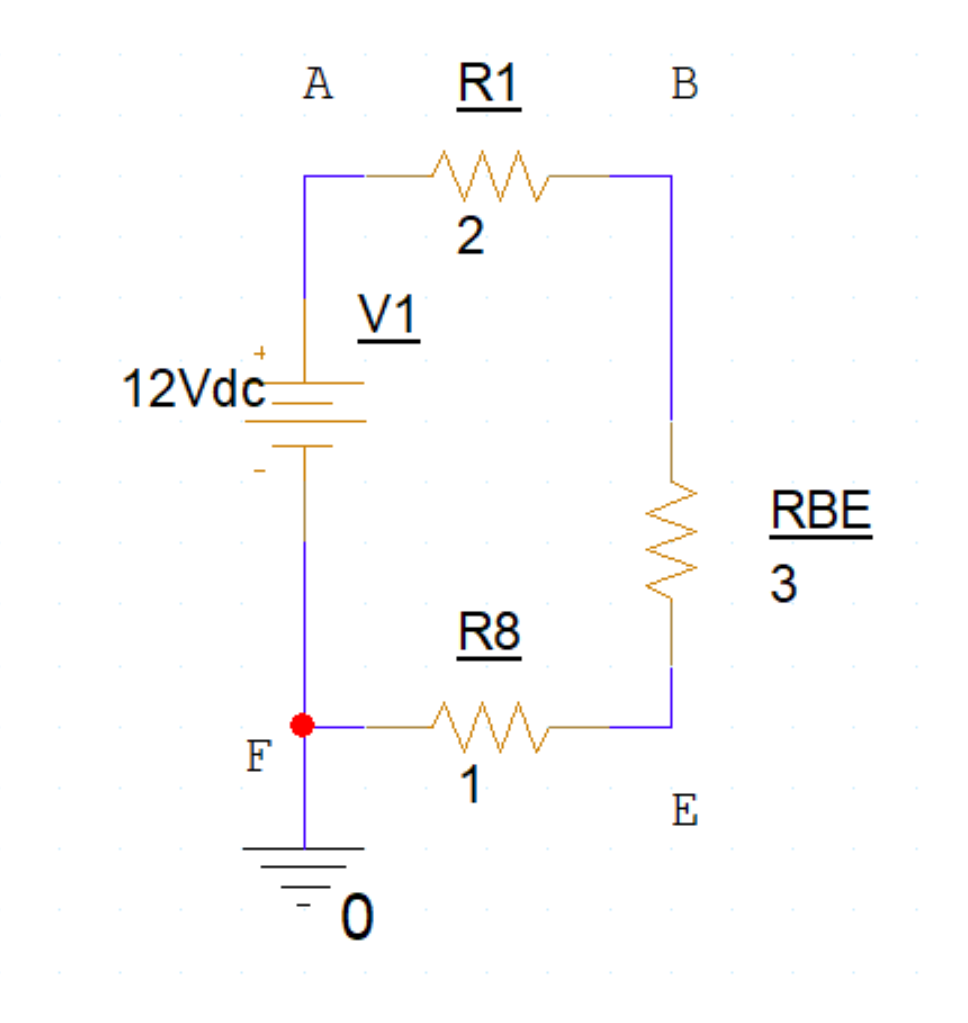
\includegraphics[width = 3in]{graphics/ex2/f5.png}
    \caption{EFET validation}
\end{figure}

A dc sweep simulation with V3 can be performed. The simulation results with V3 varies from -1V to 5V are presented as following:
\begin{figure}[!htp]
    \centering
    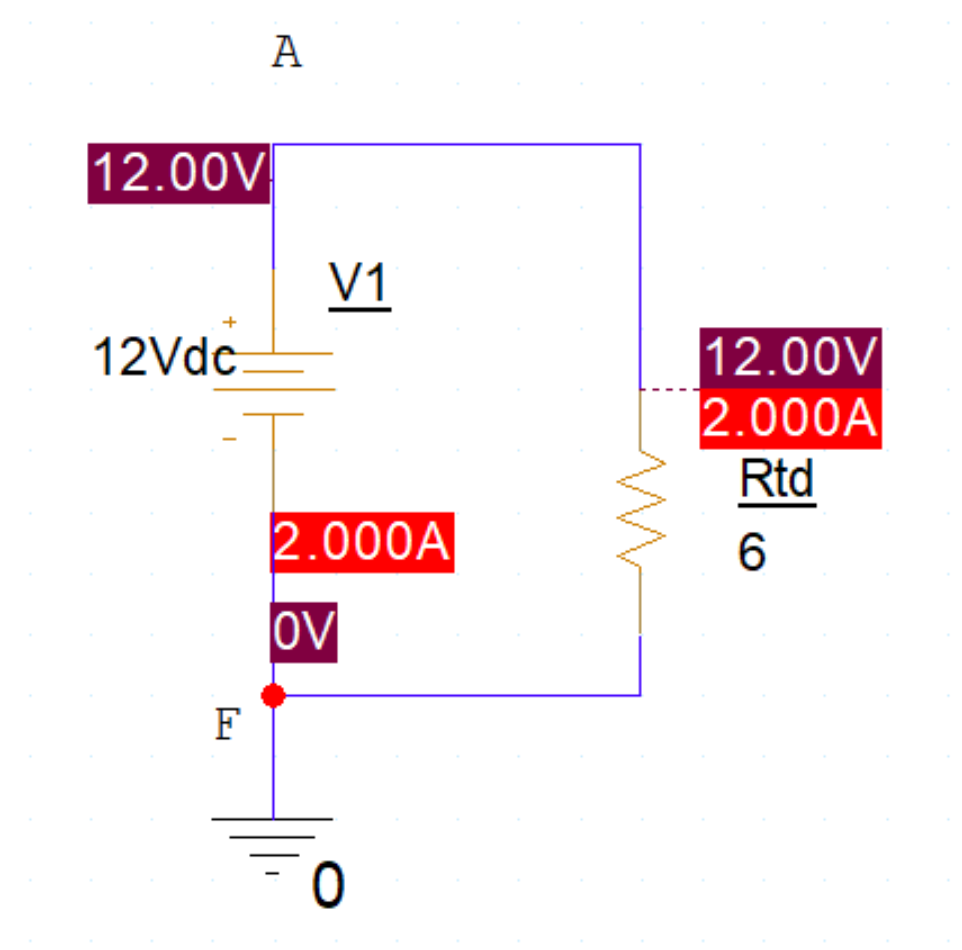
\includegraphics[width = 4.5in]{graphics/ex2/f6.png}
    \caption{Simulation results with EFET}
\end{figure}
\section{Exercise 3}
Cho sơ đồ mạch điện sau, vẽ lại mạch sao cho mạch thể hiện rõ sự nối tiếp và/hoặc song song giữa các điện trở. Sau đó tính điện trở tương đương giữa A và F, điện thế tại A, B, C, D và E. Cuối cùng, sử dụng mô phỏng để kiểm tra phép tính.
\begin{figure}[!htbp]
    \centering
    \includegraphics[width=0.7\textwidth]{graphics/ex3/f2.PNG}
    \caption{Mạch ban đầu}
\end{figure}

\subsection{Vẽ lại mạch}

\begin{figure}[!htbp]
    \centering
    \includegraphics[width=1\textwidth]{graphics/ex3/f1.PNG}
    \caption{Mạch tương đương}
\end{figure}

\pagebreak

\subsection{Tính toán}

\begin{align*}
    R_{DE} & = \frac{(R_4 + R_5)R_9}{R_4 + R_5 + R_9} = 2 \text{k}\Omega                            \\
    R_{CE} & = \frac{(R_{DE} + R_3)R_6}{R_{DE} + R_3 + R_6} = 4 \text{k}\Omega                      \\
    R_{BE} & = \frac{(R_{CE} + R_2) R_{10}}{R_{CE} + R_{2} + R_{10}} = 3 \, \text{k}\Omega.         \\
    R_{BF} & = \frac{(R_{BE} + R_{7}) R_{8}}{R_{BE} + R_{7} + R_{8}} = 3 \, \text{k}\Omega.         \\
    R_{AF} & = R_{1} + R_{BF} = 5 \, \text{k}\Omega.                                                \\ \\
%
    V_{AF} & = R_{AF} I_1 = 90 \, \text{V}.                                                         \\
    V_{BF} & = R_{BF}I_1 = 54 \, \text{V}.                                                          \\
    V_{EF} & = \frac{R_{7}}{R_{BE} + R_{7}} V_{BF} = 40.5 \, \text{V}.                               \\
    V_{BE} & = V_{BF} - V_{EF} = 13.5 \, \text{V}.                                                        \\
    V_{CF} & = \frac{R_{CE}}{R_{2} + R_{CE}} V_{BE} + V_{EF} = 49.5 \, \text{V}.                             \\
    V_{DF} & = \frac{R_{DE}}{R_{DE} + R_{3}} \frac{R_{CE}}{R_{2} + R_{CE}} V_{BE} + V_{EF} = 42 \, \text{V}. \\
\end{align*}
%
Cho \(V_F = 0\)
%
\begin{align*}
    V_{A} & = 90 \, \text{V}.   \\
    V_{B} & = 54 \, \text{V}.   \\
    V_{C} & = 49.5 \, \text{V}. \\
    V_{D} & = 42 \, \text{V}.   \\
    V_{E} & = 40.5 \, \text{V}. \\
\end{align*}

\pagebreak

\subsection{Mô phỏng}

\begin{figure}[!htbp]
    \centering
    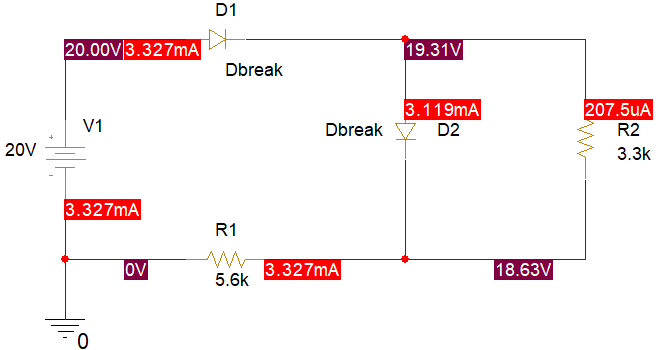
\includegraphics[width=1\textwidth]{graphics/ex3/f3.PNG}
    \caption{Mạch ban đầu}
    \includegraphics[width=1\textwidth]{graphics/ex3/f4.PNG}
    \caption{Mạch tương đương}
\end{figure}


\section{PNP Circuit}
Figure \ref{lab3_ex6_de} shows a very typical PNP transistor circuit.
Calculate $I_B$, $I_E$, and $I_C$ then simulate the circuit to double-check your calculation. Assume the current gain $\beta$ = 100.

\begin{figure}[H]
    \centering
    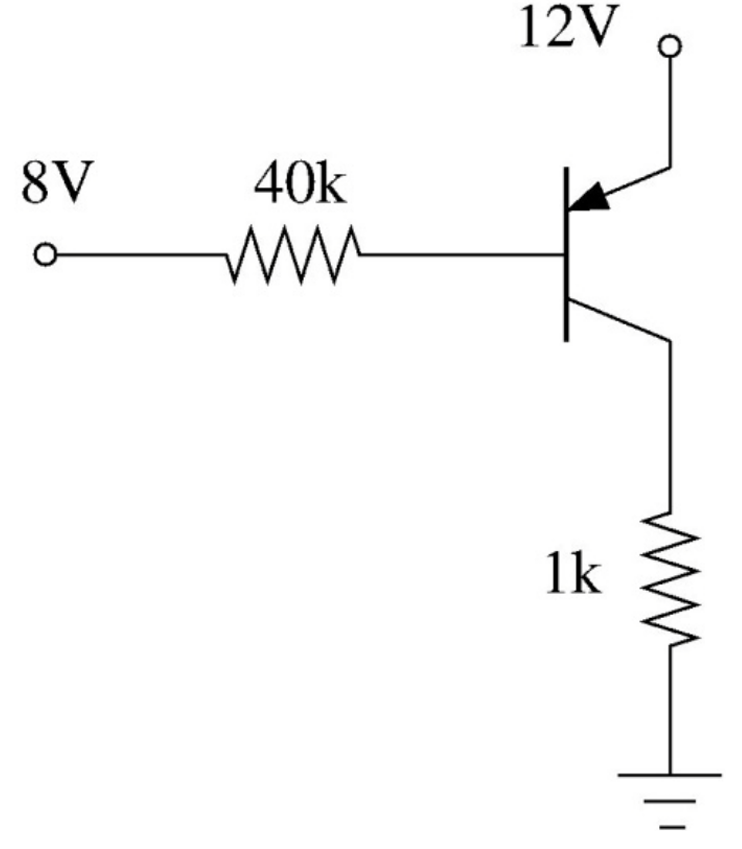
\includegraphics[width=0.5\linewidth]{graphics/ex6/f1.png}
    \caption{A PNP Circuit}
    \label{lab3_ex6_de}
\end{figure}

\subsection{Theoretical calculation}
\textit{\textbf{Notes:}}\\
\textit{Explanations, formulas, and equations are expected rather than only results.}

\begin{itemize}
    \item Vì đây là PNP transistor, nên $V_{EB}$ = 0.7 V (tránh nhầm lẫn với $V_{BE}$ trong NPN transistor).
    \item Áp dụng KVL: $$V_{EE} - V_{BB} - V_{EB} = I_B \times R_B $$
    $$ => I_B = \frac{V_{EE} - V_{BB} - V_{EB}}{R_B} = \frac{12V - 8V - 0.7V}{40k \Omega} = 82.5 \mu A $$
    \item $I_C = \beta \times I_B = 100 \times 82.5 \mu A = 8.25 mA $
    \item $I_E = I_B + I_C = 82.5\mu A + 8.25mA = 8.3325 mA$
\end{itemize}

\subsection{Simulation}
% \textbf{\textit{Your image goes here}}
\begin{figure}[H]
    \centering
    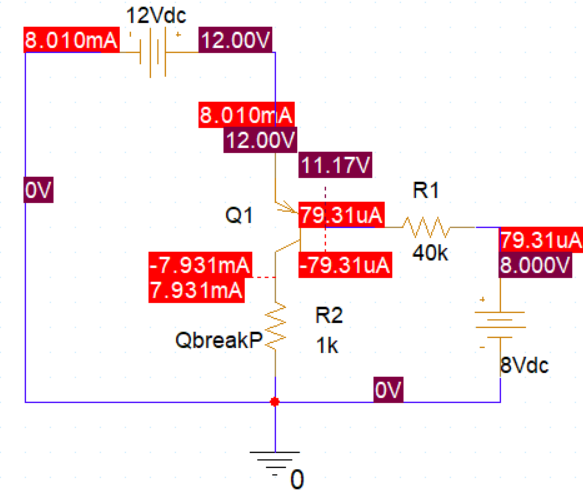
\includegraphics[width=0.9\linewidth]{graphics/ex6/f2.png}
    % \caption{A PNP Circuit}
\end{figure}

\subsection{Comparison}
$I_B$ (lý thuyết) = \dotfill$82.5 \mu A$ \dotfill $I_B$ (mô phỏng) =\dotfill $79.31 \mu A$\dotfill\bigskip\\
$I_C$ (lý thuyết) = \dotfill$ 8.250 mA$\dotfill $I_C$ (mô phỏng) = \dotfill $7.931mA$\dotfill\bigskip\\
$I_E$ (lý thuyết) = \dotfill$8.3325 mA$\dotfill $I_E$ (mô phỏng) = \dotfill$8.010mA $\dotfill\bigskip\\

\section{BJT's logic gate application}
Figure \ref{lab3_notGate_de} describes a straightforward NOT gate theoretical implementation using an NPN bipolar junction transistor. In the circuit, the NPN junction transistor operates in the saturation mode.

\begin{figure}[H]
    \centering
    % \includegraphics[width=10cm]{source/picture/bai_3/lab3_notGate_de.png}
    \caption{NPN theoretical NOT gate}
    \label{lab3_notGate_de}
\end{figure}

V1 = 0  When the source is off, the voltage would be 0V.\\
V2 = 5  When the source is on, the voltage would be 5V.\\
TD = 0  Delay time. This exercise assumes that there is no delay.\\
TR = 5ns  The rise time of the pulse (from off to on stage).\\
TF = 3ns  The fall time of the pulse (from on to off stage).\\
PW = 50ms  Pulse width: The time in which the source keeps on.\\
PER = 100ms  The period of the signal.\\

\textbf{\textit{Tips:}}\\
\\
To get the Voltage Pulse Source component in the PSpice for TI, go to \textbf{\textit{Place -> Pspice Compoment... -> Source -> Voltage Sources -> Pulse.}}

\end{document}